\section{Preparations and Flight Day}

The balloon launch base in Timmins, Ontario is located at 48.47\si{\degree}N 81.33\si{\degree}W and ALI arrived at the base located at the Victor M. Power Airport on August 25, 2014 with a launch window from September 8 to 14, 2014. In between the arrival and launch ALI had to be verified to have survived transportation, a seal within the CCD needed to be removed, thermal insulation was to be added, and finally ALI needed to be integrated onto the CNES CARMEN-2 gondola. ALI was unpacked at set up on a test bench at the launch facility and a visual inspection occurred to verify that no obvious damage occurred to the instrument during transportation. Once completed, ALI was connected to its electronics and and power boxes and power was enabled to the ALI and a local computer was used to connect to the device and verify that the system powered on correctly and that the science operation program was activated during startup. At this point it was verified that no functional problems occurred to the device during transportation, all temperature and voltage sensors, GPS module, and CCD camera were reporting diagnostic values as expected. Once the ALI system was verified to be operational an imaging check was performed to check on the optical components survived the trip. A EIA 1956 resolution target was illuminated by a 250~W tungsten halogen light source and was imaged by ALI to verify the optical layout. The recorded images were very similar to the one taken in the laboratory before the leaving Saskatoon.

Following the successful test of ALI a few final preparations were needed prior to beginning integration with CARMEN-2. First, The instrument CCD had a sealed chamber that was in a vacuum state designed to be at one atmosphere of pressure and would be required to be unsealed before the flight. The unsealing is done in order to not develop a strong pressure gradient between the CCD chamber and the low pressure 35~km environment causing permanent damage to the CCD detector itself. At the launch facility ALI was taken to a semi-clean area to unseal the CCD chamber. A panel was removed on the side of the camera and the seal to be removed can be seen in \autoref{fig:5.1:ccdVacuumUnsealing}. The orange o-ring was removed with associated sealing components and the vacuum seal was broken. The chamber panel was replaced and ALI was move back to the integration hall and another set of test resolution targets were taken to verify the correct operation of the ALI. All resolution target looked similar with from the set before the chamber was unsealed expect there was approximately a 5\% drop in counts which was excepted of the device.

\begin{figure}
    \center
    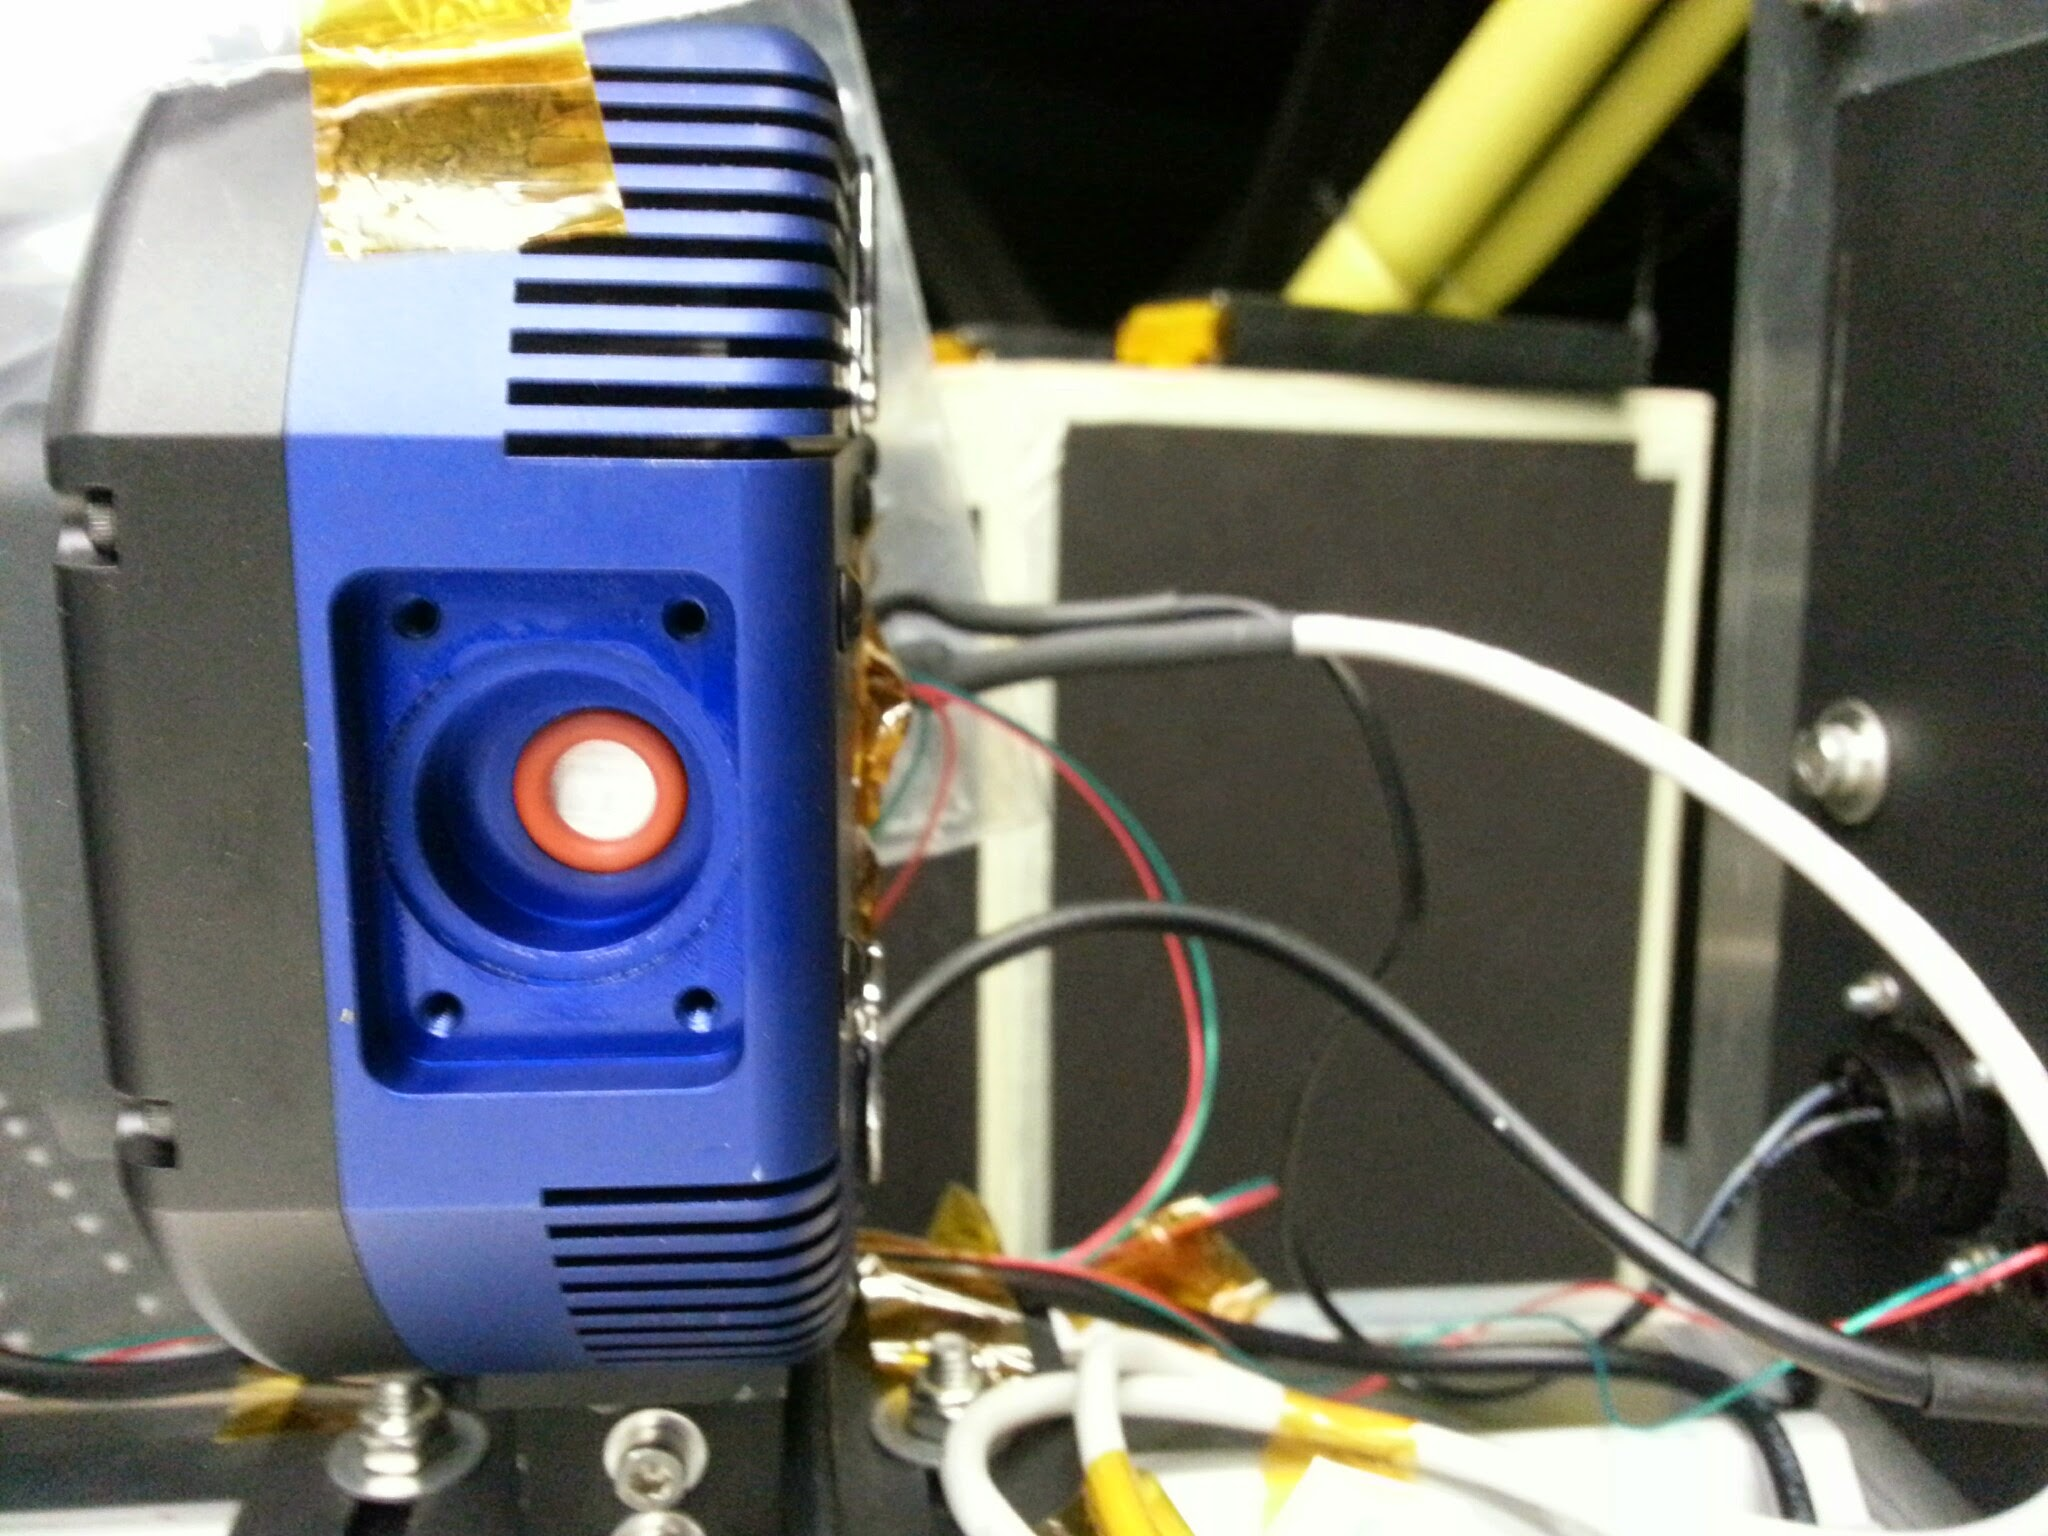
\includegraphics[trim={0 150 1200 0},clip,width=0.5\textwidth]{./Images/5-1-CCDVacuumUnsealing.jpg}
    \caption[QSI CCD Vacuum Sealing O-ring]{Side of the QSI CCD with the panel that contains the vacuum seal opened. The orange o-ring removed seen in the cavity is removed from the chamber to open the vacuum seal to the camera's CCD chip.}
    \label{fig:5.1:ccdVacuumUnsealing}
\end{figure}

 After the competition of the verification of the ALI system, work was done in order to protect ALI from the thermal environment at approximately 35~km. The first concern was the instrument reaching a temperature that was too cold to function. The instrument would have to spend some time during the initial rise in complete darkness which would result in little to no solar heating as well as pass through the tropopause where temperature can be as cold as -70\si{\degree C}. Insulation, in the form of Styrofoam, was added around the exterior of the instrument to help give ALI some thermal isolation from the environment. A second concern was once CARMEN-2 was at float altitude ALI would have to be able to survive the direct heating from the sun's radiation. The impact of the sun's energy was reduced on ALI by adding a thermal reflector to the outside of the thermal insulation expect to come into contact with the sun's radiation to reduce effects from direct heating which could cause overheating in either the optical chain or electronics boxes. The reflectance material was supplied by the CNES CARMEN-2 team and the full system with thermal management component can be seen in \autoref{fig:5.1:aliIntigratedOnCarmen}.

 \begin{figure}
    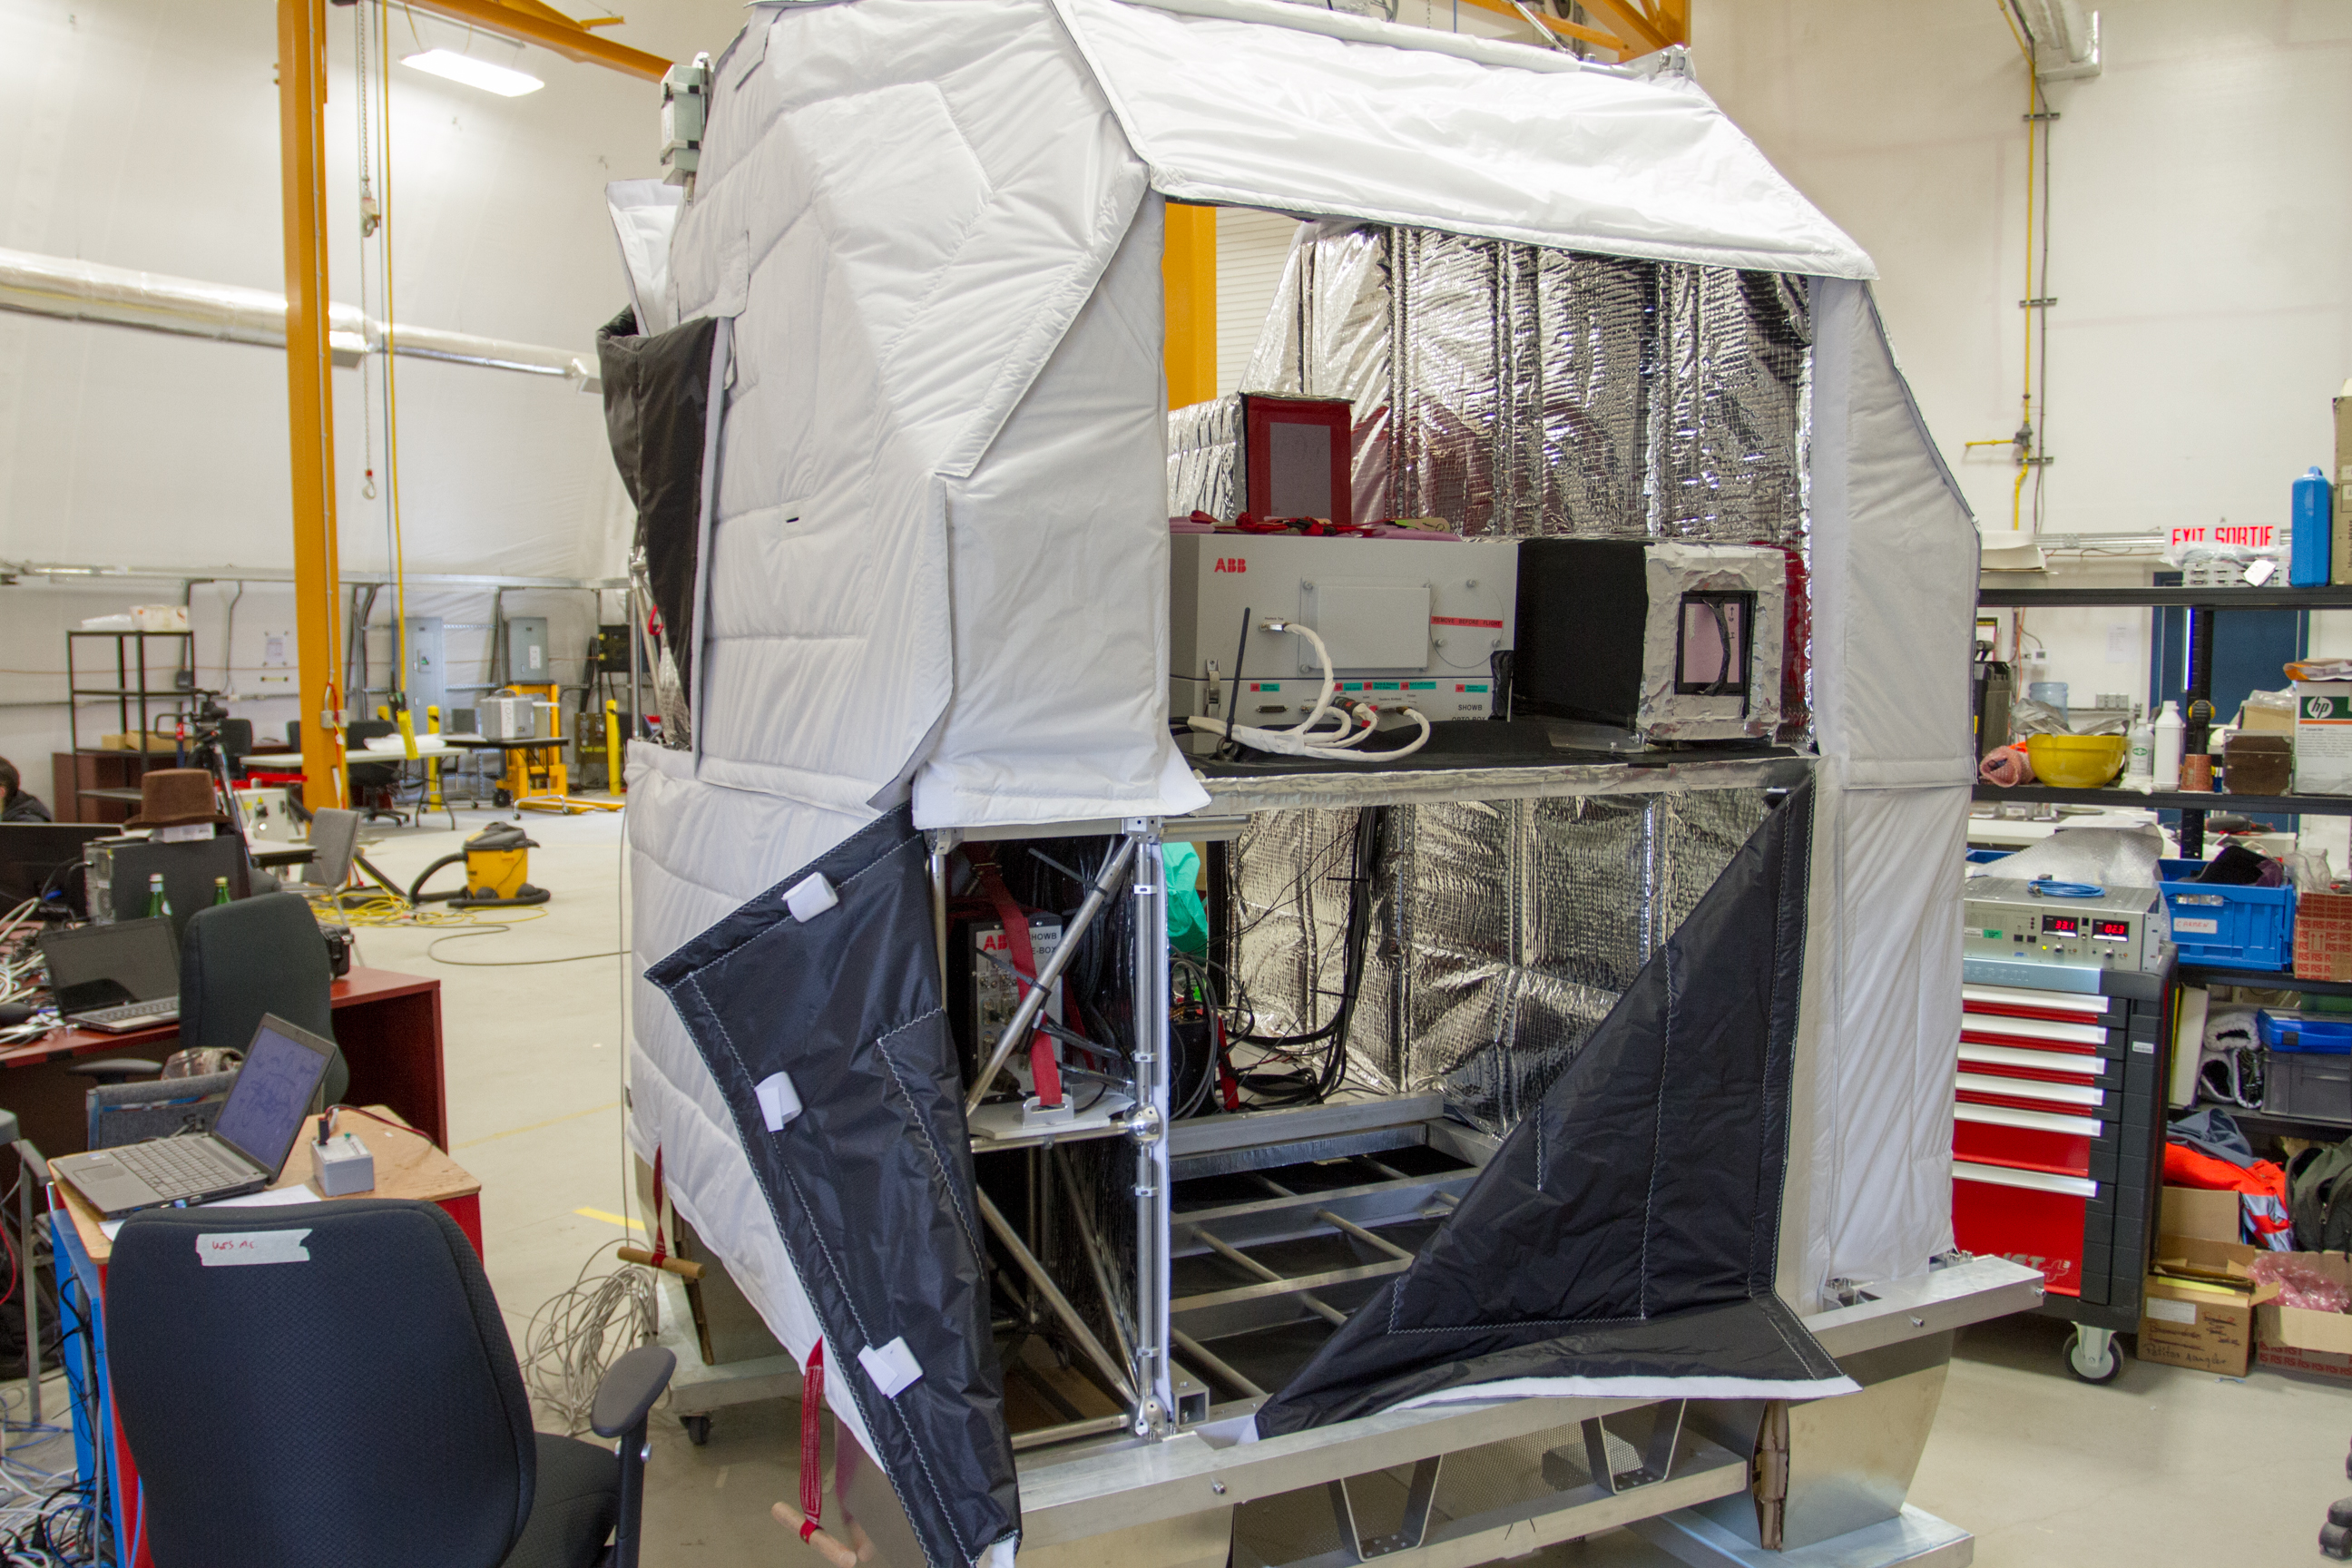
\includegraphics[trim={900 800 500 0},clip,width=0.7\textwidth]{./Images/5-1-AliIntegratedOnCarmen.jpg}
    \caption[ALI Mounted onto the CARMEN-2 Gondola]{The ALI instrument is mounted on board the CARMEN-2 gondola located next to SHOW, another Canadian instrument with collaboration between ABB, York University, and the University of Saskatchewan. Ali has its red tag cover over the optical entrance to protect the instrument from dust and other contaminates. Thermal insulation has been added to the instrument and during the flight sun side will be on the side of SHOW. Some of the reflective layer was blacked out to not cause additional stray light into SHOW optical path. With this geometry ALI will be pointed primarily to the south during the mission at approximately 90\si{\degree} from the sun.}
    \label{fig:5.1:aliIntigratedOnCarmen}
\end{figure}

After the completion of the thermal management, work was done to verify that ALI worked with the CARMEN-2 control systems and to be mounted to the gondola. Connections were verified for power and communication lines to integrate onto the CARMEN-2 system. Power lines operated as expected with no problems and there was no issues with the internal communication. However, when connection with ALI was attempted between the ground station no connection could be established. The external communication system known as the Siren module used a different ethernet setup that was used in the lab to establish a connection. Modifications were made to the flight and ground software to account for the Siren requirement and the system was retested, this time with full connection and little for UPD data losses, of which some are expected due to the nature of UDP communication. After verification ALI was mounted, with the help of the CARMEN-2 team, onto the gondola in preparation of the balloon flight. During this integration phase it should be noted that several instruments were also being verified with the CARMEN-2 systems for integrated onto the gondola including four other Canadian instruments, including a modification to the OSRIS Development model, and SHOW to measure water vapour.

The CARMEN-2 gondola itself is a pointed gondola that is piloted from the ground station in Timmins, in the case of communication failure occurs the balloon can also be piloted by a backup team located in France. The general pointing of the system is done by the CARMEN-2 control systems and once control is established a French star tracker, ESTADIOS, is used in order to further fine tune the pointing of the gondola with better to 1\si{\degree} accuracy.

The flight plan for the CARMEN-2 gondola was to have a near sunrise launch and once altitude was reached ALI, OSIRIS, and SHOW would preform their operational missions for the first four hours of the campaign followed by a scan in the azimuth direction for instrument sensitivity for ALI. During this time ALI would preform several primary mission operations including a dark imaging suite for calibration purposes, an aerosol imaging suite for aerosol measurements, and during then azimuth scan an alternative aerosol mode was run to check for angular sensitively with respect to solar location. Secondary goals were to test the sensitivity of ALI to measure water vapour and A band oxygen which is not covered in this work. After the end of the ALI mission the instrument was to be powered off and other instrument were to gather measurements.

The flight of CARMEN-2 was delayed due to poor weather conditions during the launch window. On September 20, 2014 at 05:35 UTC (01:35 local time) ALI was launched as the Nimbus 7 mission onboard the CNES CARMEN-2 gondola from the CSA Timmins balloon launch facility. During the launch, the sky was clear with light winds allowing for an safe and uneventful launch however due to the local weather conditions and forecasted weather the mission had a launch much earlier than initially anticipated. This meant that CARMEN-2 would reach float altitude and would be in the eclipse of the earth rather than viewing the sunlit atmosphere which lead to a change in the mission plan. Instead of ALI, OSIRIS, and SHOW would be on standby, still acquiring images,  during the first two hours at float while the gondola was in darkness and the star tracker would perform a segment of their mission objectives then once the sun rose the flight plan for ALI would commence.

The ascent of CARMEN-2 occurred in darkness and reached its flight altitude of 36.5~km at 8:17 UTC. First light was observed by ALI at 9:39 UTC and recorded measurements until 14:42 UTC when the primary aerosol mission was completed. ALI was powered off at 17:15 UTC during this time ALI recorded measurements for secondary goals and an azimuth scan. A visualization of the flight path with all major landmarks noted can be found on \autoref{fig:5.1:nimbus7FlightPath}. Temperature profiles for the ambient atmosphere and instrument can be seen in \autoref{fig:5.1:nimbus7Temps}. The black curve is the ambient atmospheric temperature surrounding the gondola during the flight from the ECMWF \citep{Molteni1996}. The blue, green, and red are from temperature sensors onboard ALI located on the baffle, camera, and RF driver respectively. The baffle temperature sensor was attached just on the inside of the ALI right by the entrance aperture for the system and monitors the temperature at the front of the system. The camera sensor is attached to the back of the CCD camera and the RF driver sensors measures the temperature of the RF driver. ALI was thermally insulated with styrofoam to keep the system warm which and from the baffle temperature sensor the effects of the extreme cold of the tropopause can be seen on the gondola at approximately six UTC. The cooling effect can even be seen on the interiors camera sensor and RF driver sensor which are more isolated from the exterior temperature. After, the internal temperature of the system stays at an equilibrium temperature until the sun light comes into contact on the instrument at approximately ten UTC at which point there is an increases in the systems temperature, with the aid of the reflective material heating was kept to a safe level during the flight. 

During the mission, ALI ran in two primary operational science modes, a dark mode and a aerosol imaging mode. The first mode, the dark mode was primarily used during assent and intermittently between aerosol modes. During this mode the filtering of the AOTF is disabled, meaning with no RF signal being applied to the crystal, and as such the wavelength has no dependance on the images. Eight exposures are taken at with 0.05, 0.1, 0.5, 1, 2, 3, 5, 10 second exposure times with the camera shutter operating. The second operational mode was the aerosol mode and it records 13 measurements which each consisted of a pairs of images. A pair of images, one with the AOTF enabled and one disabled, were gathered for every 25~nm between 650 to 950~nm each measurement set took approximately 25~s to acquire. The exposure times were determined by making ground based measurements of all of the wavelengths in the aerosol mode at a variety of exposure times. This data was used to determine the value at which the well of the CCD well would be three quarters full on the ground. Then using the known geometry from the ground and assumed geometry from the balloon in combination with the SASKTRAN model, which will be discussed in \autoref{TODO:??} the balloon exposure times that were used during the flight were determine which was discussed in \autoref{sec:3.3:SystemTesting}. However during the flight it was determined that the calculated exposure times were not long enough and the CCD well was not receive enough incoming radiances so the exposure time curve was recalibrated during the flight using the image statics data that are send down in the house keeping. A comparison of the two exposure time curves with the percent increase can be seen in \autoref{TODO:Make Figure}. This difference is believe to be caused by the initial exposure time calibration curves being calculated with simulated scaler radiance since the SASKTRAN polarization module had not yet been completed development. The other two science modes used during the flight for water vapour and oxygen will not be discussed but their routines during flight as well as further details on the used routines can be found in \autoref{sec:B.2:ScienceModes}. % A unique feature of the AOTF is that the diffraction can be disabled to take an image with the filter disabled. These so called `dark images' allows capture of the stray light which are use in processing to accurately and easily remove stray light from the signal, as such a `dark image' was also gathered in between each filter acquisition for assist in the calibration of the measurements.


\begin{figure}
    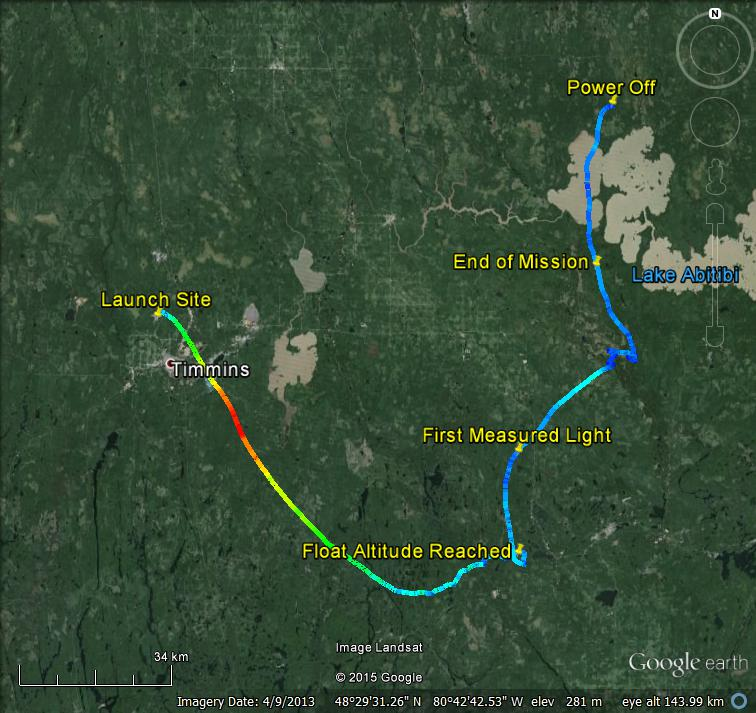
\includegraphics[width=1.0\textwidth]{./Images/5-1-AliGpsDataGoogleMaps.jpg}
    \caption[Flight Path of the Nimbus 7 Mission]{The GPS data from ALI during the Nimbus 7 mission generated via Google Earth. The colour of the line represents the absolute speed of the gondola during the mission. Important landmarks noted on the image. The end of mission represent the end of the primary aerosol mission. No GPS data was collected from ALI after the power down.}
    \label{fig:5.1:nimbus7FlightPath}
\end{figure}

\begin{figure}
    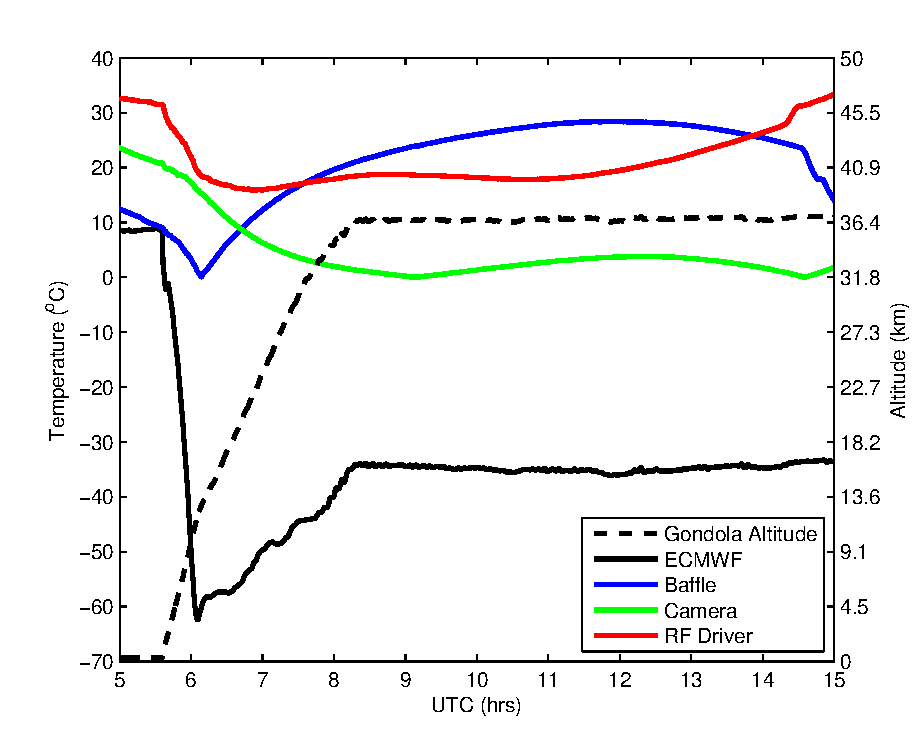
\includegraphics[width=1.0\textwidth]{./Images/5-1-FlightTemperatures.pdf}
    \caption[Flight Temperatures and Altitude Profiles from Nimbus 7]{Temperature and altitude profiles from the NIMBUS 7 flight.}
    \label{fig:5.1:nimbus7Temps}
\end{figure} 

After the completion of the mission, ALI was powered off at 17:15 UTC. The gondola continued its flight until 21:54 UTC, a 16 hour 19 minute flight, at which point it landed approximately 70~km from Amos, Quebec or approximately 250~km from the launch facility . CARMEN-2 was recovered by the balloon recovery team and was return to base on September XX, 2015. It was removed from the gondola, repacked and travelled back to Saskatoon, Saskatchewan were processing of the data occurred. 